

Theorems that comes in handy

frozen-in flux

$E = -v \times B$

\subsection{The Solar Wind and Interplanetary magnetic field}

The solar wind can be modelled by the Parker Solar model. This model suggest that the Sun is not in hydrostatic equilibrium. Using \matref{eq:mo} it is possible to show that plasma can stream out from the sun and hence create the solar wind. 

\begin{align}
\rho \frac{\partial v}{\partial t} + \rho (\vec{v} \cdot \nabla )\vec{v} = -\nabla p + \rho \vec{g}
\label{eq:mo}
\end{align}


As the pressure is dominating the particles must accelerate outward. This allows for two solutions for the problem. One that gives subsonic particle speeds at Earth and one that gives supersonic speeds at Earth. As the observed speeds are supersonic this only allows one solution. 


\subsection{Bow Shock}

When the Solar wind hits the Earth it is flowing at supersonic. Due to the magnetic field and the atmosphere of the Earth it need to slow down to subsonic speeds.This happens in a bow shock created  in front of the magnetic field. 


\subsection{Reconnection}

If the IMF is aligned in such a way that it is opposite the Earth's magnetic field reconnection is possible. \fixme{input figure for reconnection} The reconnection of the magnetic field lines as shown in \figref{fig:rec}

\begin{wrapfigure}{r}{0.4\textwidth} 
\vspace{-30pt}
  \begin{center}
    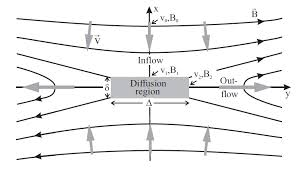
\includegraphics[width=0.4\textwidth]{Figures/reconnection.jpg}
    \caption{Sweet-Parker magnetic reconnection}
    \label{fig:rec}
  \end{center}
  \vspace{-30pt}
  \vspace{1pt}
\end{wrapfigure}


Because there is a difference in field strength between the IMF and the Earth's magnetic field the Chapman-Ferraro current is set up to balance the sides. When there is enough pressure the diffusion processes starts which results in reconnection of the magnetic field lines. 




\subsection{Dungey cycles}

As there is a reconnection on the day side the field line is stretched from the dayside to the nightside and therefore does also the plasma and field line foot move. As the fieldlines reconnects on the nightside the fieldlines and the plasma moves to the dayside again. 


\subsection{Hall, Pedersen and Birkeland currents}


Birkeland currents or Field Aligned Currents are currents that flow along the magnetic field lines. 


\subsection{Magnetic Storms}

The magnetic storm consists of two parts this is the main phase and the recovery phase. 

In the main phase the magnetic field strength drops and the Kp rises.

While in the recovery phase the magnetic field strength slowly builds up again. 


 

